\documentclass{exam}
\usepackage[utf8]{inputenc}
\usepackage{lmodern}
\usepackage{microtype}

% \usepackage[parfill]{parskip}
\usepackage[dvipsnames]{xcolor}
\usepackage{amsmath}
\usepackage{amsfonts}
\usepackage{amsthm}
\usepackage{siunitx}
\DeclareSIUnit\year{yr}
\DeclareSIUnit\foot{ft}
\DeclareSIUnit\litre{\liter}

\usepackage{skull}

\usepackage{pgfplots}
\usepgfplotslibrary{polar}
\pgfplotsset{compat=1.11}
\usepgfplotslibrary{statistics}
\usepackage{graphicx}
\usepackage{sidecap}
\sidecaptionvpos{figure}{c}
\usepackage{float}
\usepackage{gensymb}
\usepackage{tkz-euclide}
\usetkzobj{all}
\usepackage{commath}
\usepackage{hyperref}
\usepackage{enumitem}
\usepackage{wasysym}
\usepackage{multicol}
\usepackage{mathtools}
\usepackage{tcolorbox}
\usepackage{tabularx}
\usepackage[version=4]{mhchem}
\usepackage{changepage}
\usepackage{listings}
\lstset{basicstyle=\ttfamily\linespread{0.8}\small}

\renewcommand*{\thefootnote}{\fnsymbol{footnote}}

\newtheorem*{thm}{Theorem}
\newtheorem*{iden}{Identity}
\newtheorem*{lemma}{Lemma}
\newtheorem{obs}{Observation}
\theoremstyle{definition}
\newtheorem*{defn}{Definition}
\newtheorem*{ex}{Example}
\newtheorem{con}{Construction}
\newtheorem*{alg}{Algorithm}

\newtheoremstyle{break}
  {\topsep}{\topsep}%
  {\itshape}{}%
  {\bfseries}{}%
  {\newline}{}%
\theoremstyle{break}
\newtheorem*{bthm}{Theorem}

% russian integral
\usepackage{scalerel}
\DeclareMathOperator*{\rint}{\scalerel*{\rotatebox{17}{$\!\int\!$}}{\int}}

% \DeclareMathOperator*{\rint}{\int}

\pgfplotsset{vasymptote/.style={
    before end axis/.append code={
        \draw[densely dashed] ({rel axis cs:0,0} -| {axis cs:#1,0})
        -- ({rel axis cs:0,1} -| {axis cs:#1,0});
    }
}}

% \pointsinrightmargin
\boxedpoints
\pointname{}

\newcommand{\questioA}{\question[\texttt{\textbf{\color{Cerulean} A}}]}
\newcommand{\questioM}{\question[\texttt{\textbf{\color{PineGreen} M}}]}
\newcommand{\questioE}{\question[\texttt{\textbf{\color{WildStrawberry} E}}]}
\newcommand{\questioS}{\question[\texttt{\textbf{\color{Goldenrod} S}}]}
\newcommand{\questioO}{\question[\texttt{\textbf{\color{BurntOrange} O}}]}

\newcommand{\parA}{\part[\texttt{\textbf{\color{Cerulean} A}}]}
\newcommand{\parM}{\part[\texttt{\textbf{\color{PineGreen} M}}]}
\newcommand{\parE}{\part[\texttt{\textbf{\color{WildStrawberry} E}}]}
\newcommand{\parS}{\part[\texttt{\textbf{\color{Goldenrod} S}}]}
\newcommand{\parO}{\part[\texttt{\textbf{\color{BurntOrange} O}}]}

\newcommand{\subparA}{\subpart[\texttt{\textbf{\color{Cerulean} A}}]}
\newcommand{\subparM}{\subpart[\texttt{\textbf{\color{PineGreen} M}}]}
\newcommand{\subparE}{\subpart[\texttt{\textbf{\color{WildStrawberry} E}}]}
\newcommand{\subparS}{\subpart[\texttt{\textbf{\color{Goldenrod} S}}]}
\newcommand{\subparO}{\subpart[\texttt{\textbf{\color{BurntOrange} O}}]}

\newcommand{\mainHeader}[2]{\section*{NCEA Level 2 Mathematics\\#1. #2}}
\newcommand{\mainHeaderHw}[2]{\section*{NCEA Level 2 Mathematics (Homework)\\#1. #2}}
\newcommand{\seealso}[1]{\begin{center}\emph{See also #1.}\end{center}}
\newcommand{\drills}[1]{\begin{center}\emph{Drill problems: #1.}\end{center}}
\newcommand{\basedon}[1]{\begin{center}\emph{Notes largely based on #1.}\end{center}}


\begin{document}

\mainHeaderDiff{1}{The Derivative}

What is the derivative?
\begin{itemize}
  \item A way to find the slope of another function.
  \item A function giving a rate of change.
  \item A way to find maxima and minima of a function.
\end{itemize}
Essentially, the value of the derivative of a function at a point is the gradient/slope/rate of change of that function at that point.

\begin{ex}
  Consider a function defined by $ y = 2x + 1 $. At every point, the slope of the graph of this function is 2; so
  the value of the derivative of this function is 2 at every point.
\end{ex}

\begin{ex}
  The speed of a particle at any time is the rate of change of the displacement of the particle at that time;
  this can also be viewed as the slope of the displacement-time graph of the particle. Hence the speed of the
  particle is the derivative of the displacement.
\end{ex}

\begin{ex}
  In the diagram, the derivative of the red functions is shown as the blue function. Note
  that the derivative of the function depends only upon the shape, not the $ y$-shift. Also,
  see that the derivative is positive as the function increases and is negative when the
  function is decreasing. The derivative is zero exactly where the function is `flat'.

  \begin{center}
    \fbox{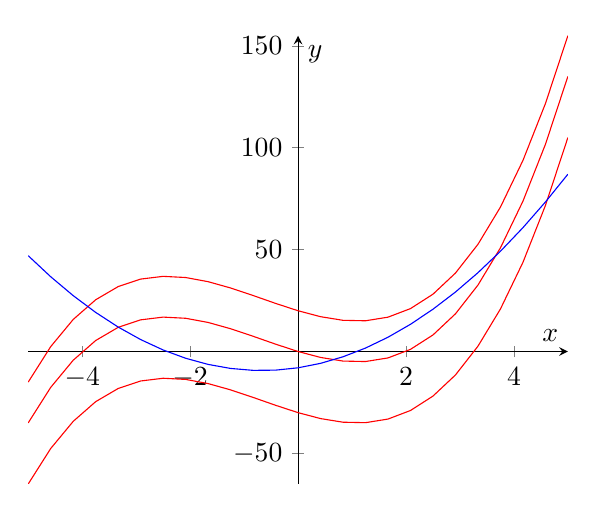
\begin{tikzpicture}
      \begin{axis}[
        axis lines = center,
        xlabel = $ x $,
        ylabel = $ y $
      ]
        \addplot[domain = -5:5, color = red] {(x - 2)*(x)*(x + 4)};
        \addplot[domain = -5:5, color = red] {(x - 2)*(x)*(x + 4) - 30};
        \addplot[domain = -5:5, color = red] {(x - 2)*(x)*(x + 4) + 20};
        \addplot[domain = -5:5, color = blue] {3*x^2 + 4*x - 8};
      \end{axis}
    \end{tikzpicture}}
  \end{center}
\end{ex}

\clearpage
\subsection*{Questions}
\begin{questions}%\item
  \questioA Why does the derivative not depend on the $ y$-shift of a function?
  \questioA Draw the derivative of each graphed function.
    \begin{multicols}{2}
    \begin{parts}
      \part
        \fbox{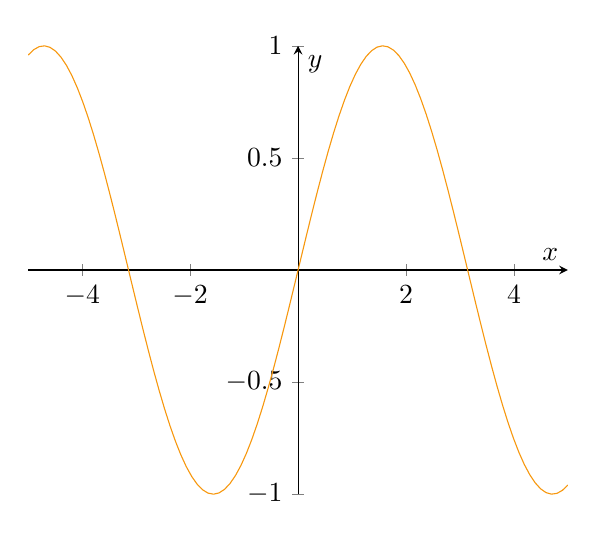
\begin{tikzpicture}
          \begin{axis}[
            axis lines = center,
            xlabel = $ x $,
            ylabel = $ y $
          ]
            \addplot[domain = -5:5, color = YellowOrange, samples=100] {sin(deg(x))};
          \end{axis}
        \end{tikzpicture}}
      \part
        \fbox{\begin{tikzpicture}
          \begin{axis}[
            axis lines = center,
            xlabel = $ x $,
            ylabel = $ y $
          ]
            \addplot[domain = -5:5, color = green] {-x^2 + 2};
          \end{axis}
        \end{tikzpicture}}
      \part
        \fbox{\begin{tikzpicture}
          \begin{axis}[
            axis lines = center,
            xlabel = $ x $,
            ylabel = $ y $
          ]
            \addplot[domain = -5:5, color = red, samples=100] {0.02*x^5 - 0.5*x^3 + x^2 - sin(x)};
          \end{axis}
        \end{tikzpicture}}
      \part
        \fbox{\begin{tikzpicture}
          \begin{axis}[
            axis lines = center,
            xlabel = $ x $,
            ylabel = $ y $
          ]
            \addplot[domain = -5:5, color = blue, samples=100] {ln(x^2)};
          \end{axis}
        \end{tikzpicture}}
    \end{parts}
    \end{multicols}

  \questioA Consider each of these functions in turn. Where is the derivative of each (i) negative, (ii) positive, (iii) zero, and (iv) undefined?
    \begin{parts}
      \part $ x \mapsto x^2 $
      \part $ x \mapsto \sin x $
      \part $ x \mapsto \tan x $
    \end{parts}
  \questioA Describe the derivative of the function $ x \mapsto \tan^{-1} x $.
  \questioM Consider the function $ f : t \mapsto \mathrm{floor}(t) $. Where is $ f $ differentiable? (Define $ \mathrm{floor}(t) $ to be the greatest integer
            less than or equal to $ t $.)
  \questioM When a hot water tap is turned on, the temperature $ T $ of the water depends on how long
            the water has been running.
    \begin{parts}
      \part Sketch a possible graph of $ T $ as a function of the time $ t $ that the tap has been running.
      \part Describe how the rate of change of $ T $ with respect to (wrt) $ t $ varies as $ t $ increases.
      \part Sketch a graph of the derivative of $ T $ wrt $ t $.
    \end{parts}
  \questioM The rate of change of a population at a time $ t $ is directly proportional to the
            population $ P(t) $ at that time, such that $ \od{P}{t} = P $. Draw a graph of the
            population over time if $ P(0) \approx 1000 $.
  \questioM Consider a continuous function $ f : \mathbb{R} \to \mathbb{R} $ which has $ n $ roots
            (all of multiplicity one) in some interval $ I $. How many roots must its derivative have
            in $ I $?
  \questioM If a function is periodic, with a period of $ T $, what can you say about its derivative?
  \questioM Consider an ellipse, $ \frac{x^2}{a^2} + \frac{y^2}{b^2} = 1 $. This is not a function: since both $ (0, b) $ and $ (0, -b) $ are
            members of the function, it fails the vertical line test. However, it would be nice to reason about its
            rate of change \textit{as if it were} a function. Describe the slope of the ellipse as a particle traces the curve in
            an anticlockwise direction at a constant rate.
  \questioM The number of bacteria after $ t $ hours in a controlled laboratory experiment is $ n = f(t) $.
    \begin{parts}
      \part What is the meaning of the derivative $ f'(5) $? What are its units?
      \part Suppose that there is an unlimited amount of space and nutrients. Which would you
            expect to be larger, $ f'(5) $ or $ f'(10) $? If the supply of nutrients is limited
            does your answer change?
    \end{parts}
\end{questions}
\end{document}
